\documentclass[10pt]{article}
\usepackage[letterpaper,margin=0.85in]{geometry}
\usepackage[T1]{fontenc}
\usepackage{lmodern}
\usepackage{microtype}
\usepackage{amsmath,amssymb}
\usepackage{booktabs}
\usepackage{graphicx}
\usepackage{subcaption}
\usepackage{enumitem}
\usepackage{xcolor}
\usepackage[labelfont=bf,font=small]{caption}
\usepackage[colorlinks=true,linkcolor=black,citecolor=black,urlcolor=blue!50!black]{hyperref}
\graphicspath{{figs/}}
\setlist{nosep,leftmargin=1.4em}
\setlength{\parskip}{0.35em}
\setlength{\parindent}{0pt}
\renewcommand{\topfraction}{0.9}
\renewcommand{\floatpagefraction}{0.8}
\newcommand{\MSE}{\operatorname{MSE}}
\newcommand{\RR}{\mathbb{R}}

\title{\vspace{-1.2em}\textbf{Additive Faces: Non-negative Matrix Factorization\\ versus PCA on the Olivetti Faces}\vspace{-0.2em}}
% Replace the placeholders with the group members' names.
\author{Person 1 \and Person 2 \and Person 3 \and Person 4}
\date{STOR 565, Fall 2026}

\begin{document}
\maketitle
\vspace{-1.8em}

\begin{abstract}\small
We compare non-negative matrix factorization (NMF), which writes each face as a nonnegative sum of learned patterns, with PCA on the 400 Olivetti face images. Both methods use one fixed 320/80 split, one error definition (per-pixel test MSE on unclipped reconstructions) and the same number of components. At $k=40$ the test MSE is $0.003658$ for PCA and $0.003946$ for NMF, so NMF is $7.9\%$ higher. Across initializations and stopping tolerances the gap is $5.5\%$--$7.9\%$, and NMF is above PCA at every component count we tried ($k=5,\dots,100$). The gap is not caused by PCA's mean term. The NMF patterns give an additive explanation of every reconstruction, but they are broad and overlapping, not isolated facial parts. Our evidence covers new photos of people seen in training, one split, and pixel error only.
\end{abstract}

\section{Question, data and evaluation protocol}
\textbf{Question.} NMF is a method we did not cover in class. It represents an image as an \emph{addition} of nonnegative patterns, whereas PCA (our class baseline) uses signed directions around a mean. What does the additive representation cost in reconstruction accuracy, and what does it give in interpretability?

\textbf{Data.} The Olivetti faces (AT\&T Laboratories Cambridge~\cite{samaria1994}) contain 400 grayscale photographs: 10 of each of 40 people. Our preprocessed file stores each image as 4096 pixel values ($64\times64$) in $[0,1]$, together with a fixed train/test split with 8 training and 2 test photos per person ($n_{\text{train}}=320$, $n_{\text{test}}=80$; drawn with a stratified split, seed 42). Identity labels are not used by either method.

\textbf{Protocol.} Both methods are fitted on the 320 training images only and evaluated on the same 80 test images in the original pixel space. We report the per-pixel mean squared error
\[
\MSE(X,\hat X)=\frac{\|X-\hat X\|_F^2}{nd},
\]
computed on \emph{unclipped} reconstructions (clipping to $[0,1]$ is used only for display). PCA centers with the training mean. NMF uses the raw nonnegative intensities, because subtracting a mean would create negative entries. The two methods are compared at the same number of components $k$; the main comparison uses $k=40$, the setting of our NMF implementation. One caveat shapes everything below: every person appears in both the training and the test split, so the test photos are \emph{new photos of known people}, not new people.

\section{Methods}
\subsection{PCA (baseline)}
Let $X\in\RR^{n\times d}$ be the training matrix with mean row $\mu$ and centered SVD $X-\mathbf 1\mu^\top=USV^\top$. Rank-$k$ PCA reconstructs $\hat x=\mu+(x-\mu)V_kV_k^\top$, where $V_k$ holds the first $k$ right singular vectors. By the Eckart--Young theorem~\cite{eckart1936} this is the best rank-$k$ approximation of the centered training matrix in squared error. Coefficients and directions can have either sign.

\subsection{NMF model and objective}
NMF seeks nonnegative factors
\[
X\approx WH,\qquad W\in\RR_+^{n\times k},\ H\in\RR_+^{k\times d},\qquad \hat x_i=\sum_{r=1}^{k}W_{ir}H_{r,:}.
\]
Each row of $H$ is a pattern (an image), each row of $W$ says how much of each pattern one image uses, and nothing can be subtracted. The number $k=40$ is the chosen representation size; it does not assign one component to each of the 40 people. We minimize the squared-error objective~\cite{lee2001}
\[
\min_{W\ge0,\;H\ge0}\ f(W,H)=\tfrac12\|X-WH\|_F^2,\qquad \nabla_Wf=(WH-X)H^\top,\quad \nabla_Hf=W^\top(WH-X),
\]
with no sparsity or other penalty. Training minimizes the same quantity that MSE measures, so the comparison with PCA is on the metric the objective targets.

\subsection{Optimization}
With $H$ fixed, $f$ is convex in $W$, and vice versa, but $f$ is \emph{not jointly convex}. Exact NMF is NP-hard~\cite{vavasis2008}, so no practical solver comes with a global-optimality guarantee. We use scikit-learn's~\cite{pedregosa2011} coordinate descent (\texttt{solver="cd"}, \texttt{init="nndsvda"}, \texttt{tol=1e-4}, at most 3000 sweeps, \texttt{random\_state=42}), the fast local method of Cichocki and Phan~\cite{cichocki2009} rather than the multiplicative updates of Lee and Seung~\cite{lee2001}. Fixing all entries but one, $f$ is a one-variable quadratic whose constrained minimizer is
\[
W_{ir}\leftarrow\max\Bigl(0,\;W_{ir}-\frac{(\nabla_Wf)_{ir}}{a_r}\Bigr),\quad a_r=\sum_{j}H_{rj}^2>0,
\]
and symmetrically for $H_{rj}$ with denominator $\sum_iW_{ir}^2$. Sweeping over all coordinates, alternating between $W$ and $H$, never increases $f$; stopping at the tolerance does not prove a global optimum.

\textbf{Test images.} After training, $H$ is fixed and each test image receives the nonnegative coefficients $\arg\min_{w\ge0}\|x-wH\|_2^2$ (a convex nonnegative least-squares problem); the patterns are \emph{not} refitted. We checked that scikit-learn's \texttt{transform} solves this essentially exactly: its test MSE equals the exact SciPy NNLS solution ($0.00394635$ for both, difference $7.8\times10^{-10}$).

\subsection{Two facts that frame the comparison}
\emph{(i) A bound on training error.} For every $W\in\RR^{n\times k}$, $H\in\RR^{k\times d}$, $\|X-WH\|_F\ge\|X-X_k\|_F$, where $X_k$ is the rank-$k$ truncated SVD of the \emph{uncentered} training matrix~\cite{eckart1936}. NMF factors are a special case, so NMF's training error cannot fall below this bound. PCA is a centered variant that stores one more image (the mean). These statements concern training error only; no theorem gives the same ordering on test images, so we measure it. To separate the cost of nonnegativity from the effect of the missing mean term we add two references (Table~\ref{tab:k40}): PCA with $k-1=39$ components plus the mean (40 stored images, like NMF) and the uncentered truncated SVD (no mean, signed factors).\\
\emph{(ii) Non-uniqueness.} For any positive diagonal $D$, $(WD)(D^{-1}H)=WH$, and components can be permuted, so raw coefficient sizes and component indices are not importance measures.

\section{Results}
\subsection{Matched comparison at \texorpdfstring{$k=40$}{k = 40}}
\begin{table}[!t]
\centering\small
\caption{Reconstruction error at $k=40$ (same training images, same 80 test images, unclipped).}\label{tab:k40}
\begin{tabular}{lcccc}
\toprule
Method & Mean term & Train MSE & Test MSE & Test MSE vs.\ PCA\\
\midrule
PCA, 40 components + mean & yes & 0.002796 & 0.003658 & ---\\
PCA, 39 components + mean & yes & 0.002851 & 0.003696 & $+1.0\%$\\
Uncentered SVD, 40 components & no & 0.002820 & 0.003658 & $-0.005\%$\\
NMF, 40 components & no & 0.003079 & 0.003946 & $+7.9\%$\\
\bottomrule
\end{tabular}
\end{table}
PCA has lower training and test error than NMF (Table~\ref{tab:k40}). The uncentered SVD, which has no mean term, reaches the same test error as PCA, and PCA with 39 components plus the mean still beats NMF. The NMF gap is therefore not explained by the missing mean; it reflects the nonnegativity constraint together with the fact that coordinate descent stops at a local solution (Section~\ref{sec:robust}). NMF's training MSE ($0.003079$) stays above the Eckart--Young bound ($0.002820$), as it must, and it fell monotonically at every recorded sweep count (Fig.~\ref{fig:conv}a).

The difference is not driven by a few images: PCA has the lower error on 74 of the 80 test images, and the mean paired difference (NMF$-$PCA) is $2.88\times10^{-4}$, with a 95\% percentile-bootstrap interval of $[2.33,\,3.44]\times10^{-4}$ (Fig.~\ref{fig:conv}b; 10{,}000 resamples of the 80 per-image differences). This interval reflects variation across these test images only; it does not capture variation across people or across splits. Visually the two reconstructions are very similar and both blur fine detail (Fig.~\ref{fig:recon}); a lower MSE means closer pixel values, not better identity recognition or perceptual quality.

\begin{figure}[!t]
\centering
\begin{subfigure}[t]{0.52\linewidth}\centering
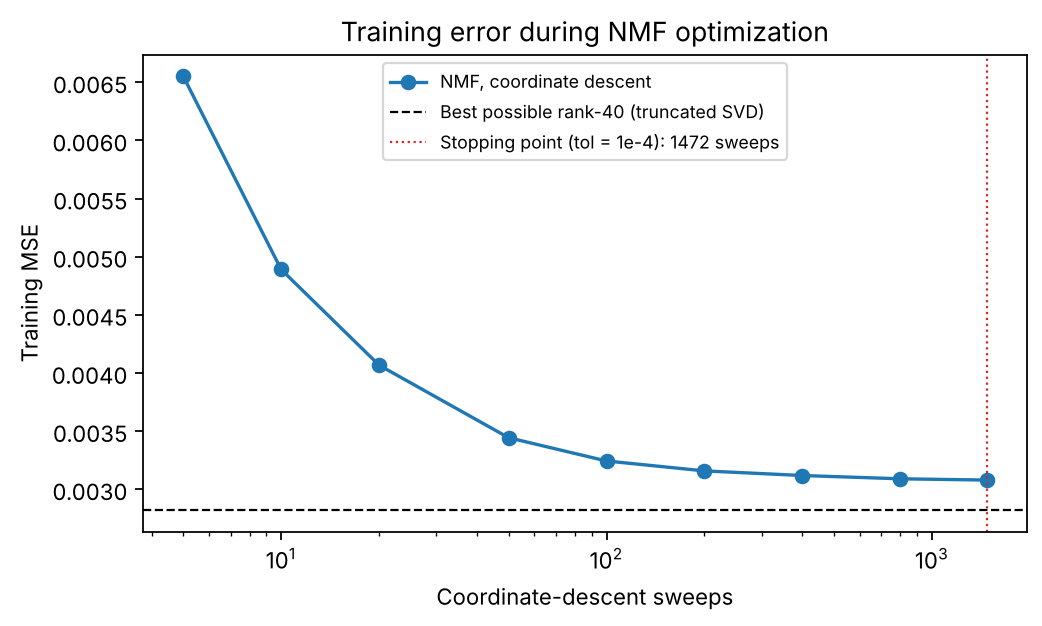
\includegraphics[width=\linewidth]{04_convergence.png}\caption{NMF training MSE versus sweeps.}
\end{subfigure}\hfill
\begin{subfigure}[t]{0.42\linewidth}\centering
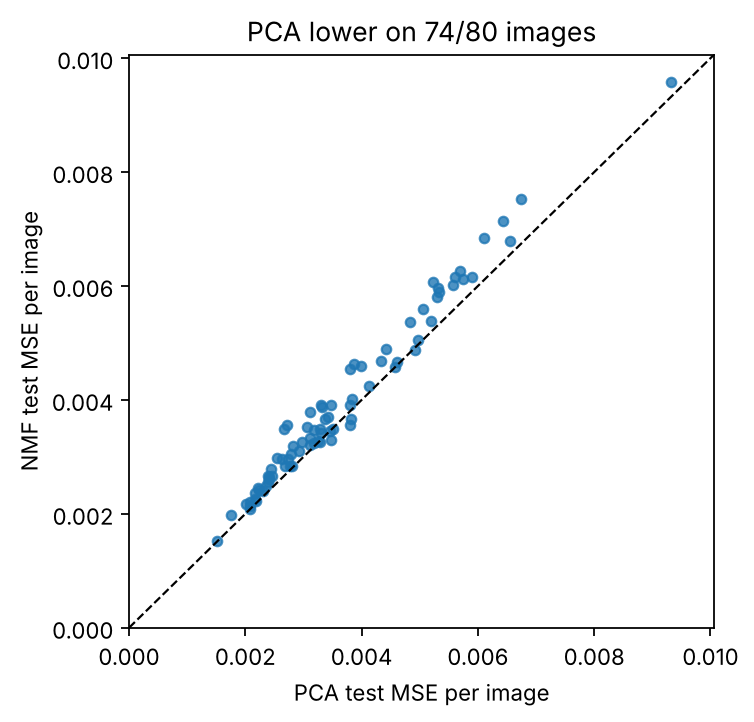
\includegraphics[width=\linewidth]{06_paired_errors.png}\caption{Per-image test MSE, NMF vs.\ PCA.}
\end{subfigure}
\caption{(a) The error falls quickly (0.00655 after 5 sweeps, 0.00324 after 100) and then slowly; the run stops at the tolerance after 1472 sweeps and stays above the best possible rank-40 error (dashed). (b) Each dot is one test image; points above the diagonal are images where PCA is better.}\label{fig:conv}
\end{figure}

\subsection{How robust is the gap?}\label{sec:robust}
\textbf{Component count.} We refit NMF with the same settings at $k=5,10,25,40,50,100$ (the grid of our PCA analysis). NMF's test error is above PCA's at every $k$, and the gap tends to grow with $k$: $+1.9\%$, $+1.9\%$, $+4.3\%$, $+7.9\%$, $+7.7\%$ and $+17.5\%$ (Fig.~\ref{fig:kgrid}). The fits at $k=50$ and $100$ stopped at the 3000-sweep limit, so their gaps are upper bounds on what NMF could reach with more sweeps; we read them as a direction, not a measurement.

\begin{figure}[!t]
\centering
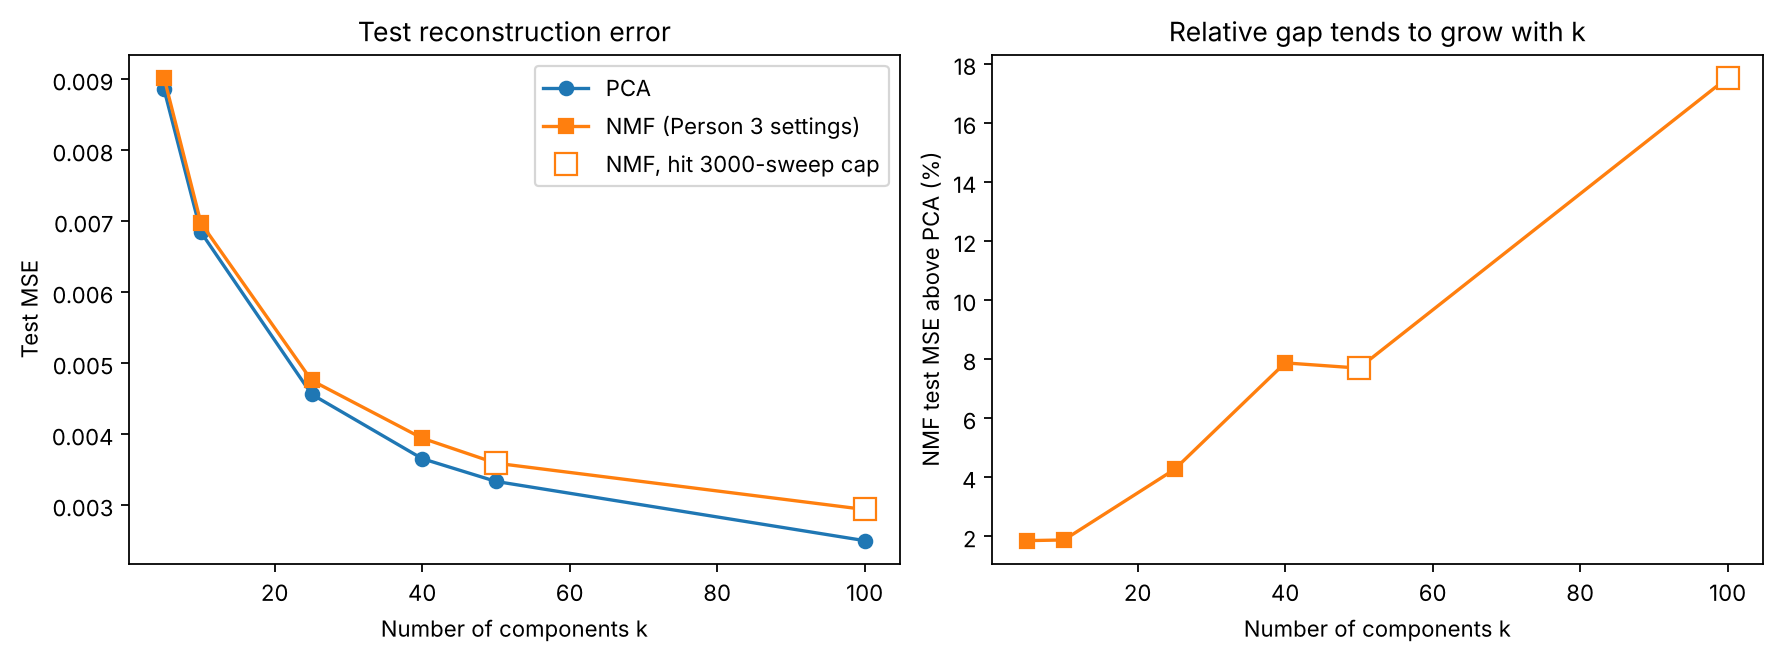
\includegraphics[width=0.86\linewidth]{07_k_grid.png}
\caption{Test MSE (left) and the relative gap of NMF over PCA (right) for $k=5,\dots,100$. Hollow markers: NMF hit the iteration limit.}\label{fig:kgrid}
\end{figure}

\textbf{Initialization and tolerance.} The $k=40$ result above is one deterministic initialization and one tolerance. Table~\ref{tab:init} refits with a stricter tolerance and five random initializations. All variants stay above PCA, but the size of the gap moves by a couple of percentage points, and the single run in Table~\ref{tab:k40} gives the largest gap. No convergence warning means the numerical criterion was met, not that the best NMF solution was found. We therefore report the gap at $k=40$ as a range, $5.5\%$--$7.9\%$.

\begin{table}[!t]
\centering\small
\caption{NMF at $k=40$ under different initializations and stopping rules (PCA test MSE $=0.003658$).}\label{tab:init}
\begin{tabular}{lccc}
\toprule
Variant & Sweeps & Test MSE & vs.\ PCA\\
\midrule
\texttt{nndsvda}, tol $10^{-4}$ (our implementation) & 1472 & 0.003946 & $+7.9\%$\\
\texttt{nndsvda}, tol $10^{-5}$, up to 6000 sweeps & 6000 (cap) & 0.003919 & $+7.1\%$\\
random init, seeds 0--4 (mean $0.003874$, sd $1.5\times10^{-5}$) & 3000 (cap) & 0.003859--0.003899 & $+5.5\%$ to $+6.6\%$\\
\bottomrule
\end{tabular}
\end{table}

\subsection{What do the patterns look like?}
Figure~\ref{fig:comp} shows the first eight stored components of each model. NMF patterns are nonnegative images that overlap and remain largely face-like (for example, NMF 3 emphasizes the forehead and NMF 6 is dominated by a bright strip along the left image boundary, yet both contain broader facial structure), whereas PCA components are signed contrasts. We quantify ``broad and overlapping'' with Hoyer's sparsity measure~\cite{hoyer2004}, $(\sqrt d-\|v\|_1/\|v\|_2)/(\sqrt d-1)$, which is 0 for a flat vector and 1 for a single nonzero pixel. The mean sparsity of the 40 NMF patterns is $0.317$ (range $0.22$--$0.52$), only modestly above that of PCA's absolute loadings ($0.221$, a descriptive reference only), and far from 1. About $18.7\%$ of the entries of $H$ and $25.5\%$ of the training coefficients are exactly zero, so a typical training image still uses $29.8$ of the 40 patterns. In the first test image, split into its 40 additive contributions, the largest one supplies only $11.4\%$ of the total brightness and the top 20 supply $87\%$, so no single pattern dominates. Nonnegativity therefore guarantees an additive explanation, but it did not produce a small set of localized parts here; Lee and Seung~\cite{lee1999} report parts-based face representations; our patterns are much broader, so we do not reproduce a clean parts-based result.

\begin{figure}[!t]
\centering
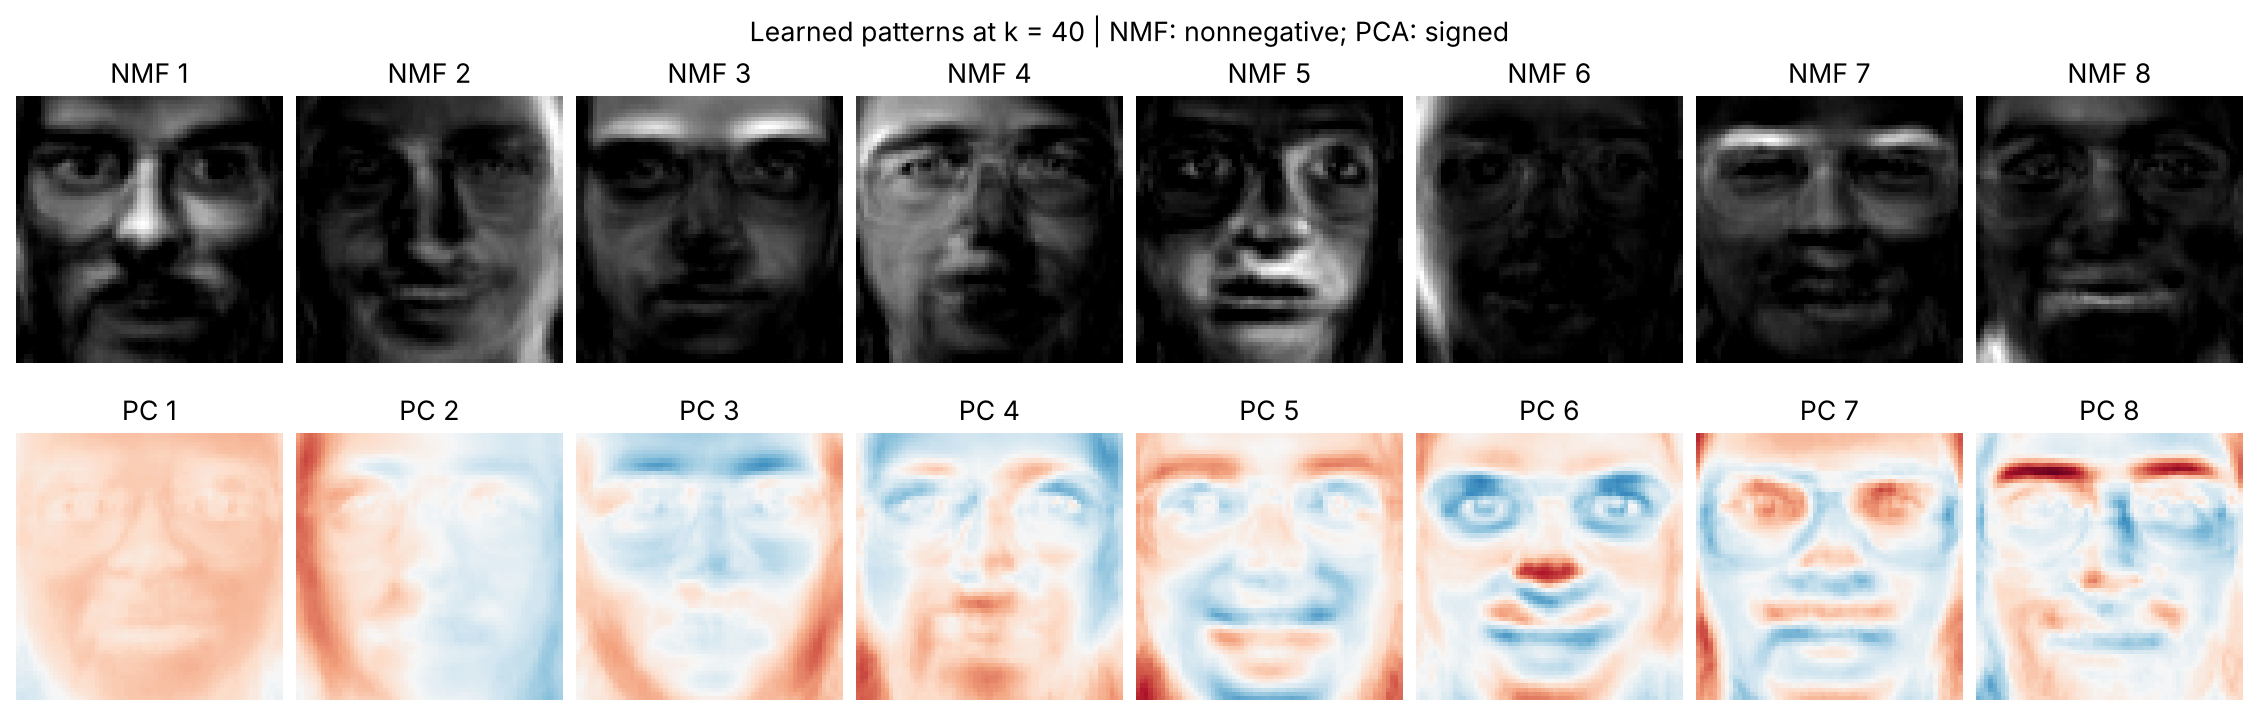
\includegraphics[width=\linewidth]{01_components.png}
\caption{First eight stored components at $k=40$. NMF patterns are each scaled by their own maximum for display only; PCA components share a symmetric color scale (red positive, blue negative). Columns of the two rows do not correspond.}\label{fig:comp}
\end{figure}

\begin{figure}[!t]
\centering
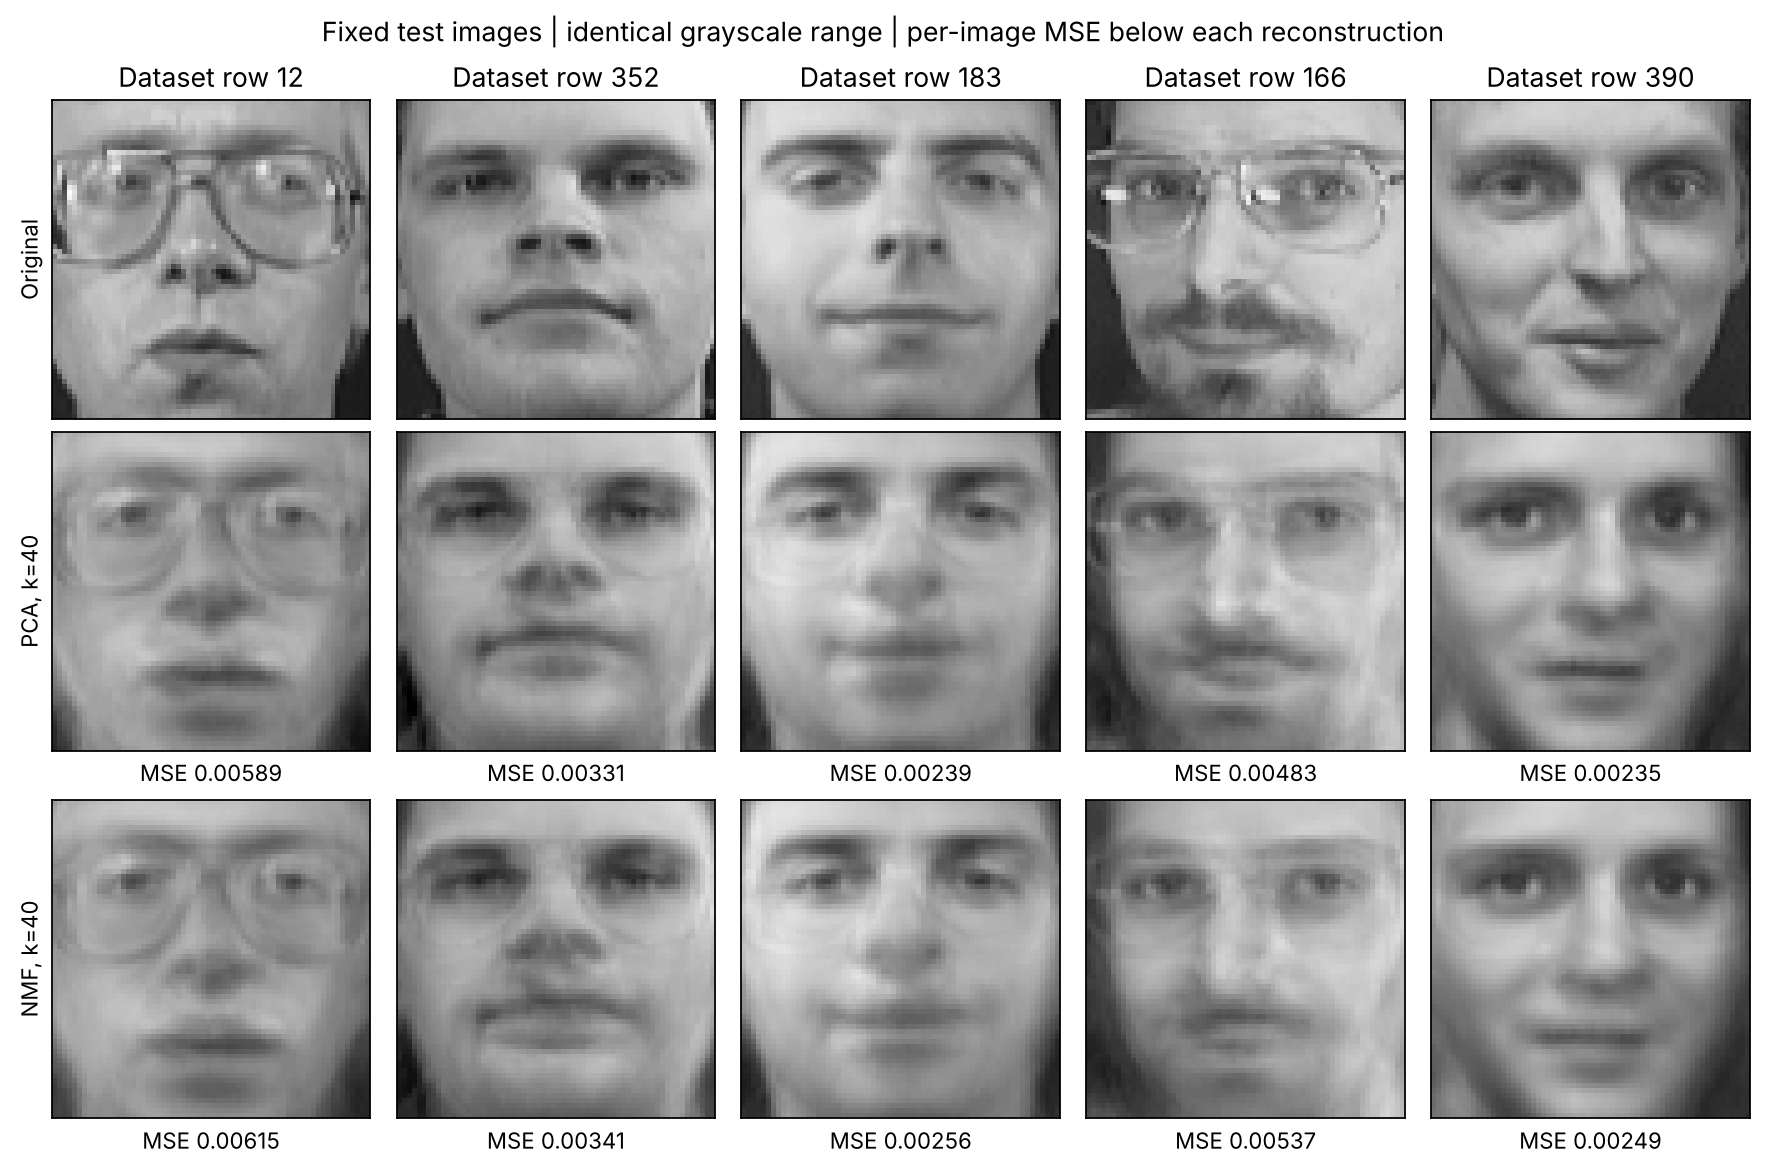
\includegraphics[width=0.6\linewidth]{03_matched_reconstructions.png}
\caption{Five fixed test images and their $k=40$ reconstructions, with per-image MSE. NMF's relative gap is largest for row 166 ($+11.2\%$) and smallest for row 352 ($+3.2\%$).}\label{fig:recon}
\end{figure}

\section{Interpretation and limitations}
\textbf{What the evidence supports.} On this split, at matched $k$, PCA reconstructs held-out photos of known people better than NMF in every variant we ran, on most individual images, and at every component count tried, and the gap is not due to the mean term. NMF's advantage is that every reconstruction is a sum of nonnegative contributions that can be inspected; here that advantage is modest because the patterns are broad.\\
\textbf{Limitations.}
\begin{enumerate}[label=\arabic*.]
\item \emph{Local optimization.} Different initializations and tolerances give different solutions and gaps (Table~\ref{tab:init}); an NMF run is an upper bound on what the model class can achieve. The fits at $k=50,100$ were capped at 3000 sweeps.
\item \emph{Non-unique factors.} Scaling and permutation (Section~2.4) mean coefficient sizes and component order are not absolute. Donoho and Stodden~\cite{donoho2003} study when a decomposition into parts is identifiable; we did not check their conditions.
\item \emph{Additive is not localized.} We did not test sparsity-promoting or spatially constrained variants~\cite{hoyer2004}, which may behave differently.
\item \emph{Population and split.} Every identity appears in both splits, so results concern new photos of known people; unseen identities would need a subject-disjoint split. We use one split and no validation set, so the intervals describe test-image variation only.
\item \emph{One metric.} MSE does not measure interpretability, recognition accuracy or perceptual quality, and PCA's optimality is a training-error statement that does not guarantee lower error on every unseen image.
\end{enumerate}

\section{Conclusion}
NMF represents a face as a nonnegative weighted sum of learned patterns; coordinate descent fits the training factors, and test encoding adjusts only the coefficients, which we verified is solved essentially exactly. The price relative to PCA is higher pixel error ($+5.5\%$ to $+7.9\%$ at $k=40$, tending to grow with $k$), a nonconvex training problem and non-unique factors. The gain is a direct additive reading of every reconstruction, but nonnegativity alone did not yield independent facial parts. We do not claim that one method is universally better or that these results extend to unseen people.

\section{Reproducibility}
Code, data and a README are in one repository: \url{https://github.com/MachineWJQ6657/pca-vs-nmf}. The notebook \texttt{STOR565\_Project\_Combined.ipynb} runs top to bottom in 7 to 9 minutes on one CPU thread and writes all tables and figures; it contains the original PCA and NMF parts of Persons 1--3 (unchanged apart from marked edits) and the analysis above, and it checks that the parts agree on every shared number (for example, PCA at each shared $k$ and NMF at $k=40$ to relative tolerance $10^{-8}$). The data file \texttt{data/olivetti\_preprocessed.npz} has SHA-256 \texttt{85be2275\ldots4eef}; \texttt{make\_data.py} compares it with the public Olivetti data and reproduces the split exactly. All fits use fixed seeds and a one-thread BLAS limit. The numbers here were produced with Python 3.13, NumPy 2.5, SciPy 1.18 and scikit-learn 1.9.

\clearpage
\begin{thebibliography}{99}\small
\bibitem{lee1999} D.~D. Lee and H.~S. Seung. Learning the parts of objects by non-negative matrix factorization. \emph{Nature}, 401(6755):788--791, 1999.
\bibitem{lee2001} D.~D. Lee and H.~S. Seung. Algorithms for non-negative matrix factorization. In \emph{Advances in Neural Information Processing Systems 13}, 2001.
\bibitem{cichocki2009} A.~Cichocki and A.-H. Phan. Fast local algorithms for large scale nonnegative matrix and tensor factorizations. \emph{IEICE Trans.\ Fundamentals}, E92-A(3):708--721, 2009.
\bibitem{donoho2003} D.~Donoho and V.~Stodden. When does non-negative matrix factorization give a correct decomposition into parts? In \emph{Advances in Neural Information Processing Systems 16}, 2003.
\bibitem{vavasis2008} S.~A. Vavasis. On the complexity of nonnegative matrix factorization. arXiv:0708.4149, 2008.
\bibitem{hoyer2004} P.~O. Hoyer. Non-negative matrix factorization with sparseness constraints. \emph{Journal of Machine Learning Research}, 5:1457--1469, 2004.
\bibitem{eckart1936} C.~Eckart and G.~Young. The approximation of one matrix by another of lower rank. \emph{Psychometrika}, 1(3):211--218, 1936.
\bibitem{pedregosa2011} F.~Pedregosa et al. Scikit-learn: Machine learning in Python. \emph{Journal of Machine Learning Research}, 12:2825--2830, 2011.
\bibitem{samaria1994} F.~S. Samaria and A.~C. Harter. Parameterisation of a stochastic model for human face identification. In \emph{Proceedings of the Second IEEE Workshop on Applications of Computer Vision}, Sarasota, FL, 1994. Face images courtesy of AT\&T Laboratories Cambridge.
\end{thebibliography}

\section*{Contribution statement}
\small
\textbf{Person 1:} data preprocessing and the first PCA run ($k=50$). \textbf{Person 2:} PCA analysis ($k=5,\dots,100$, components, reconstructions, error tables). \textbf{Person 3:} NMF implementation at $k=40$ (patterns, reconstructions, train/test MSE). \textbf{Person 4:} NMF theory and analysis (model and optimization, convergence and exact test-encoding checks, reference models, robustness over $k$ and initialization, sparsity, limitations). The merged notebook, this report and the slides were prepared with AI assistance (see the appendix).

\clearpage
\section*{Appendix: AI-use statement}
\small
\textbf{Tool.} Claude (Anthropic) was used throughout the Person~4 work and for assembling the final notebook, report and slides.

\textbf{What we delegated.} Review of the Person~4 notebook against the course requirements and against the notebooks of Persons~1--3; the extra analyses in the NMF part (convergence curve, exact test-encoding check, uncentered-SVD and 39-component reference models, paired bootstrap, sparsity, component-count grid, initialization study); merging the four parts into one notebook; translating the Chinese text of Person~3's notebook into English; drafting the README, this report and the slides.

\textbf{What we kept.} The data file and split; the code and results of Persons~1--3 (verified unchanged, apart from two edits the group approved: the English translation of Person~3's text, and one \texttt{print} statement that no longer writes an absolute file path); the choice of topic, of $k=40$ and of the evaluation protocol; the decision about which claims the report makes; and the responsibility for the submission.

\textbf{Three checks.}
\begin{enumerate}[label=\arabic*.]
\item \emph{Math and sources.} The Eckart--Young statement used in Section~2.4 was tested numerically: NMF's training MSE ($0.003079$) stays above the truncated-SVD bound ($0.002820$) at every recorded sweep. Reference titles, authors, venues and pages were checked against publisher, arXiv or archive pages; the pages of Lee and Seung (2001) and of Samaria and Harter (1994) could not be confirmed and are omitted.
\item \emph{Code and data.} The original notebooks of Persons~1--3 were re-run independently and reproduce their reported numbers (PCA $k=50$ test MSE $0.003337$; the PCA table for $k=5,\dots,100$; NMF $k=40$: 1472 sweeps, test MSE $0.00394635$). The split was reproduced exactly from its recipe. An automated comparison of the code syntax trees confirms that the merged notebook's code for Persons~1--3 is identical to the originals (only text strings and comments differ, and the one approved \texttt{print}); the check fails if even one number such as $k=40$ is altered.
\item \emph{Claims and figures.} Every sentence of the Person~4 analysis is tied to a cell that fails if the computed numbers no longer support it (18 such checks pass). Checking produced corrections: a plot caption claiming the gap ``grows with $k$'' was changed to ``tends to grow'' because the gap dips at $k=50$; a stated run time of 9 minutes was replaced by the measured time; ``most images use most patterns'' was replaced by the measured 29.8 of 40.
\end{enumerate}
\end{document}
